% !TeX TXS-program:compile = txs:///lualatex

\documentclass[a4paper,11pt]{article}
\usepackage[revgoku]{cp-base}
\graphicspath{{./graphics/}}
%variables
\donnees[%
	classe={1\up*{ère} 2M2},matiere={[SPÉ.MATHS]},mois=Novembre,annee=2021,typedoc=CHAP,numdoc=4]

%formatage
\author{Pierquet}
\title{\nomfichier}
\hypersetup{pdfauthor={Pierquet},pdftitle={\nomfichier},allbordercolors=white,pdfborder=0 0 0,pdfstartview=FitH}
%fancy
\lhead{\entete{\matiere}}
\chead{\entete{\lycee}}
\rhead{\entete{\classe{} - \mois{} \annee}}
%\rhead{\entete{\classe{} - Chapitre }}
\lfoot{\pied{\matiere}}
\cfoot{\logolycee{}}
\rfoot{\pied{\numeropagetot}}

\begin{document}

\pagestyle{fancy}

\part{CH04 - Second degré, études de signes - Exercices (Correction)}

\smallskip

\exonum{0}
%
\begin{enumerate}
	\item 
	\begin{enumerate}
		\item $4x^2-7x-3$ : $\Delta=(-7)^2-4\times4\times(-3)=97$ et les racines sont $\begin{dcases} x_1 = \frac{-b+\sqrt{\Delta}}{2a}=\frac{7+\sqrt{97}}{8} \approx 2,106 \\ x_2 = \frac{-b-\sqrt{\Delta}}{2a}=\frac{7-\sqrt{97}}{8} \approx -0,356 \end{dcases}$.
		
		\begin{center}
			\begin{tikzpicture}
				\tkzTabInit[lgt=4,espcl=2]{$x$/0.8,$4x^2-7x-3$/0.8}{$-\infty$,$x_2$,$x_1$,$+\infty$}
				\tkzTabLine{,+,z,-,z,+,}
				\aidesignetkztabPL[code=pa+d+,racines={x2/x1},couleur=blue]{1}[0.75][1.5]
			\end{tikzpicture}
		\end{center}
		\item $-7x^2+12x-6$ : $\Delta=-24$, donc pas de racine et signe $\ominus$
		
		\begin{center}
			\begin{tikzpicture}
				\tkzTabInit[lgt=4,espcl=3]{$x$/0.8,$-7x^2+12x-6$/0.8}{$-\infty$,$+\infty$}
				\tkzTabLine{,-,}
				\aidesignetkztabPL[code=pa-d-,couleur=purple]{1}[0.75][1.5]
			\end{tikzpicture}
		\end{center}
		\item $4x^2-2,4x+0,36$ : $\Delta=0$, la racine est $x_0=\dfrac{-b}{2a}=0,3$ avec le signe $\oplus$.
		
		\begin{center}
			\begin{tikzpicture}
				\tkzTabInit[lgt=4,espcl=2]{$x$/0.8,$4x^2-{2,4}x+{0,36}$/0.8}{$-\infty$,${0,3}$,$+\infty$}
				\tkzTabLine{,+,z,+,}
				\aidesignetkztabPL[code=pa+d0,racines={0,3},couleur=blue]{1}[0.75][1.5]
			\end{tikzpicture}
		\end{center}
	\end{enumerate}
	\item 
	\begin{enumerate}
		\item $-x^2+5x+7 \pg 0$ est bien une inéquation du second degré.
		
		$-x^2+5x+7 = 0$ : $\Delta=53$, les deux racines sont $x_1=\dfrac{5-\sqrt{53}}{2} \approx -1,14$ et $x_2=\dfrac{5+\sqrt{53}}{2} \approx 6,14$.
		
		\begin{center}
			\begin{tikzpicture}
				\tkzTabInit[lgt=4,espcl=2]{$x$/0.8,$-x^2+5x+7$/0.8}{$-\infty$,$x_1$,$x_2$,$+\infty$}
				\draw[black,fill=red!25] (N21) rectangle (N32);
				\tkzTabLine{,-,z,+,z,-,}
				\aidesignetkztabPL[code=pa-d+,racines={x1/x2},couleur=ForestGreen]{1}[0.75][1.5]
			\end{tikzpicture}
		\end{center}
		Ainsi, $\mathscr{S}=\intervFF{x_1}{x_2}$.
		\item $11x^2+16x-9<10x+8$ n'est pas (encore) une inéquation du second degré.
		
		Or $11x^2+16x-9<10x+8 \ssi 11x^2+16x-9-10x-8<0 \ssi 11x^2+6x-17<0$ qui est bien une inéquation du second degré.
		
		$11x^2+6x-17 = 0$ : $\Delta=784$, les deux racines sont $x_1=1$ et $x_2=\dfrac{-17}{11}$.
		
		\begin{center}
			\begin{tikzpicture}
				\tkzTabInit[lgt=4,espcl=2]{$x$/0.8,$11x^2+6x-17$/0.8}{$-\infty$,$-\nicefrac{17}{11}$,$1$,$+\infty$}
				\draw[black,fill=red!25] (N21) rectangle (N32);
				\tkzTabLine{,+,z,-,z,+,}
				\aidesignetkztabPL[code=pa+d+,racines={x2/x1},couleur=orange]{1}[0.75][1.5]
			\end{tikzpicture}
		\end{center}
		Ainsi, $\mathscr{S}=\intervOO{\dfrac{-17}{11}}{1}$.
	\end{enumerate}
\end{enumerate}

\pagebreak

\exonum{2}

\begin{enumerate}
	\item $(x-1)(x^2-5x+6)>0$ est bien \textsf{ZPQ}
	
	\tabula{}$\bullet~~x-1=0 \ssi x=1$ et le signe est $\ominus\oplus$ ;
	
	\tabula{}$\bullet~~x^2-5x+6=0$ : $\Delta=1$, les racines sont $x_1=2$ et $x_2=3$ avec le signe $\oplus\ominus\oplus$.
	
	\begin{center}
		\begin{tikzpicture}
			\tkzTabInit[lgt=4,espcl=2]{$x$/0.8,$x-1$/0.8,$x^2-5x+6$/0.8,expr/0.8}{$-\infty$,$1$,$2$,$3$,$+\infty$}
			\draw[black,fill=red!25] (N24) rectangle (N33);
			\draw[black,fill=red!25] (N44) rectangle (T23);
			\tkzTabLine{,-,z,+,t,+,t,+,}
			\tkzTabLine{,+,t,+,z,-,z,+,}
			\tkzTabLine{,-,z,+,z,-,z,+,}
			\aidesignetkztabPL[code=da+,racines={1},couleur=blue]{1}[0.75][1.5]
			\aidesignetkztabPL[code=pa+d+,racines={2/3},couleur=red]{2}[0.75][1.5]
		\end{tikzpicture}
	\end{center}
	\tabula{}$\bullet~~$ainsi $\mathscr{S}=\intervOO{1}{2} \cup \intervOO{3}{+\infty}$.
	\item $\dfrac{-x^2+5x-7}{2x+5} \pp 0$ est bien \textsf{ZPQ}
	
	\tabula{}$\bullet~~-x^2+5x-7=0$ : $\Delta=-3$, pas de racine et le signe est $\ominus$ ;
	
	\tabula{}$\bullet~~2x+5=0 \ssi x=-\tfrac52$ et le signe est $\ominus\oplus$.
	
	\begin{center}
		\begin{tikzpicture}
			\tkzTabSetup[doubledistance=2pt]
			\tkzTabInit[lgt=4,espcl=2]{$x$/0.8,$-x^2+5x-7$/0.8,$2x+5$/0.8,expr/0.8}{$-\infty$,$-{2,5}$,$+\infty$}
			\draw[black,fill=red!25] (N24) rectangle (T23);
			\draw(N21) node [yshift=1pt] {{\scriptsize \red \textsf{D}}};
			\tkzTabLine{,-,t,-,}
			\tkzTabLine{,-,z,+}
			\tkzTabLine{,+,d,-,}
			\aidesignetkztabPL[code=pa-d-,couleur=purple]{1}[0.75][1.5]
			\aidesignetkztabPL[code=da+,racines={-2,5},couleur=orange]{2}[0.75][1.5]
		\end{tikzpicture}
	\end{center}
	\tabula{}$\bullet~~$ainsi $\mathscr{S}=\intervOO{-2,5}{+\infty}$.
	\item $x^3-x^2+4x \pg 0$ n'est pas encore sous forme \textsf{ZPQ}, on transforme :
	
	$x^3-x^2+4x \pg 0 \ssi x(x^2-x+4) \pg 0$ qui est bien sous forme \textsf{ZPQ}
	
	\tabula{}$\bullet~~x=0$ et a pour signe $\ominus\oplus$ ;
	
	\tabula{}$\bullet~~x^2-x+4=0$ : $\Delta=-15$ et le signe $\oplus$.
	
	\begin{center}
		\begin{tikzpicture}
			\tkzTabInit[lgt=4,espcl=2]{$x$/0.8,$x$/0.8,$x^2-x+4$/0.8,expr/0.8}{$-\infty$,$0$,$+\infty$}
			\draw[black,fill=red!25] (N24) rectangle (T23);
			\tkzTabLine{,-,z,+,}
			\tkzTabLine{,+,t,+}
			\tkzTabLine{,-,z,+,}
			\aidesignetkztabPL[code=da+,racines={0},couleur=blue]{1}[0.75][1.5]
			\aidesignetkztabPL[code=pa+d-,couleur=purple]{2}[0.75][1.5]
		\end{tikzpicture}
	\end{center}
	\tabula{}$\bullet~~$ainsi $\mathscr{S}=\intervFO{0}{+\infty}$.
	\item $\dfrac{3x}{x+1} \pg 5x$ n'est pas encore sous forme \textsf{ZPQ}, on transforme :
	
	$\dfrac{3x}{x+1} \pg 5x \ssi \dfrac{3x}{x+1} -5x \pg 0 \ssi \dfrac{3x}{x+1}-\dfrac{5x(x+1)}{x+1} \pg 0 \ssi \dfrac{3x-5x^2-5x}{x+1} \pg 0 \ssi \dfrac{-5x^2-2x}{x+1} \pg 0$ qui est bien \textsf{ZPQ}
	
	\tabula{}$\bullet~~-5x^2-2x=0$ : $\Delta=4$, les racines sont $x_1=0$ et $x_2=-0,4$ avec le signe $\ominus\oplus\ominus$ ;
	
	\tabula{}$\bullet~~x+1=0 \ssi x=-1$ et le signe est $\ominus\oplus$.
	
	\begin{center}
		\begin{tikzpicture}
			\tkzTabSetup[doubledistance=2pt]
			\tkzTabInit[lgt=4,espcl=2]{$x$/0.8,$-5x^2-2x$/0.8,$x+1$/0.8,expr/0.8}{$-\infty$,$-1$,${-0,4}$,$0$,$+\infty$}
			\draw(N21) node [yshift=1pt] {{\scriptsize \red \textsf{D}}};
			\draw[black,fill=red!25] (T13) rectangle (N24);
			\draw[black,fill=red!25] (N33) rectangle (N44);
			\tkzTabLine{,-,t,-,z,+,z,-,}
			\tkzTabLine{,-,z,+,t,+,t,+,}
			\tkzTabLine{,+,d,-,z,+,z,-,}
			\aidesignetkztabPL[code=pa-d+,racines={x2/0},couleur=red]{1}[0.75][1.5]
			\aidesignetkztabPL[code=da+,racines={-1},couleur=ForestGreen]{2}[0.75][1.5]
		\end{tikzpicture}
	\end{center}
	\tabula{}$\bullet~~$ainsi $\mathscr{S}=\intervOO{-\infty}{-1} \cup \intervOF{-0,4}{0}$.
\end{enumerate}

\medskip

\exonum{2}

\begin{enumerate}
	\item $\dfrac{x^2-10x+25}{-5x^2-3x+8} \pp 0$ est bien sous la forme \textsf{ZPQ} :
	
	\tabula{}$\bullet~~x^2-10x+25=0$ : $\Delta=0$, la racine est $x_0=5$ avec le signe $\oplus$ ;
	
	\tabula{}$\bullet~~-5x^2-3x+8=0$ : $\Delta=169$, les racines sont $x_1=-1,6$ et $x_2=1$ avec le signe $\ominus\oplus\ominus$.
	
	\begin{center}
		\begin{tikzpicture}
			\tkzTabSetup[doubledistance=2pt]
			\tkzTabInit[lgt=4,espcl=2]{$x$/0.8,$x^2-10x+25$/0.8,$-5x^2-3x+8$/0.8,expr/0.8}{$-\infty$,${-1,6}$,$1$,$5$,$+\infty$}
			\draw(N21) node [yshift=1pt] {{\scriptsize \red \textsf{D}}};
			\draw(N31) node [yshift=1pt] {{\scriptsize \red \textsf{D}}};
			\draw[black,fill=red!25] (T13) rectangle (N24);
			\draw[black,fill=red!25] (N33) rectangle (T24);
			\tkzTabLine{,+,t,+,t,+,z,+,}
			\tkzTabLine{,-,z,+,z,-,t,-,}
			\tkzTabLine{,-,d,+,d,-,z,-,}
			\aidesignetkztabPL[code=pa+d0,racines={5},couleur=orange]{1}[0.75][1.5]
			\aidesignetkztabPL[code=pa-d+,racines={x1/1},couleur=blue]{2}[0.75][1.5]
		\end{tikzpicture}
	\end{center}
	
	\tabula{}$\bullet~~$ainsi $\mathscr{S}=\intervOO{-\infty}{-1,6} \cup \intervOO{1}{+\infty}$.
	\item $\dfrac{-2x}{x+2} \pp \dfrac{3x+2}{x-1}$ n'est pas (encore) sous la forme \textsf{ZPQ}.
	
	$\dfrac{-2x}{x+2} \pp \dfrac{3x+2}{x-1} \ssi \dfrac{-2x}{x+2}-\dfrac{3x+2}{x-1} \pp 0 \ssi \dfrac{-2x(x-1)}{(x+2)(x-1)}-\dfrac{(3x+2)(x+2)}{(x+2)(x-1)} \pp 0$.
	
	Soit encore $\dfrac{-2x}{x+2} \pp \dfrac{3x+2}{x-1} \ssi \dfrac{-2x^2+2x-3x^2-6x-2x-4}{(x+2)(x-1)} \pp 0 \ssi \dfrac{-2x}{x+2} \pp \dfrac{3x+2}{x-1} \ssi \dfrac{-5x^2-6x-4}{(x+2)(x-1)} \pp 0$ qui est bien \textsf{ZPQ} :
	
	\tabula{}$\bullet~~-5x^2-6x-4=0$ : $\Delta=-44$, pas de racine et le signe est $\ominus$ ;
	
	\tabula{}$\bullet~~x+2=0 \ssi x=-2$ et le signe est $\ominus\oplus$ ;
	
	\tabula{}$\bullet~~x-1=0 \ssi x=1$ et le signe est $\ominus\oplus$.
	
	\begin{center}
		\begin{tikzpicture}
			\tkzTabSetup[doubledistance=2pt]
			\tkzTabInit[lgt=4,espcl=2]{$x$/0.8,$-5x^2-6x-4$/0.8,$x+2$/0.8,$x-1$/0.8,expr/0.8}{$-\infty$,$-2$,$1$,$+\infty$}
			\draw(N21) node [yshift=1pt] {{\scriptsize \red \textsf{D}}};
			\draw(N31) node [yshift=1pt] {{\scriptsize \red \textsf{D}}};
			\draw[black,fill=red!25] (T14) rectangle (N25);
			\draw[black,fill=red!25] (N34) rectangle (T25);
			\tkzTabLine{,-,t,-,t,-,}
			\tkzTabLine{,-,z,+,t,+,}
			\tkzTabLine{,-,t,-,z,+,}
			\tkzTabLine{,-,d,+,d,-,}
			\aidesignetkztabPL[code=pa-d-,couleur=red]{1}[0.75][1.5]
			\aidesignetkztabPL[code=da+,racines={-2},couleur=blue]{2}[0.75][1.5]
			\aidesignetkztabPL[code=da+,racines={1},couleur=ForestGreen]{3}[0.75][1.5]
		\end{tikzpicture}
	\end{center}
	
	\tabula{}$\bullet~~$ainsi $\mathscr{S}=\intervOO{-\infty}{-2} \cup \intervOO{1}{+\infty}$.
	\pagebreak
	\item $(-x^2+5x-6)(-3x^2+5x-2) \pg 0$ qui est bien \textsf{ZPQ} :
	
	\tabula{}$\bullet~~-x^2+5x-6=0$ : $\Delta=1$, les deux racines sont $x_1=2$ et $x_2=3$ avec le signe $\ominus\oplus\ominus$ ;
	
	\tabula{}$\bullet~~-3x^2+5x-2=0$ : $\Delta=1$, les deux racines sont $x_3=\dfrac23$ et $x_4=1$ avec le signe $\ominus\oplus\ominus$.
	
	\begin{center}
		\begin{tikzpicture}
			\tkzTabInit[lgt=4,espcl=1.5]{$x$/0.8,$-x^2+5x-6$/0.8,$-3x^2+5x-2$/0.8,expr/0.8}{$-\infty$,$\nicefrac{2}{3}$,$1$,$2$,$3$,$+\infty$}
			\draw[black,fill=red!25] (T13) rectangle (N24);
			\draw[black,fill=red!25] (N33) rectangle (N44);
			\draw[black,fill=red!25] (N53) rectangle (T24);
			\tkzTabLine{,-,t,-,t,-,z,+,z,-,}
			\tkzTabLine{,-,z,+,z,-,t,-,t,-,}
			\tkzTabLine{,+,z,-,z,+,z,-,z,+,}
			\aidesignetkztabPL[code=pa-d+,racines={x4/1},couleur=red]{1}[0.75][1.5]
			\aidesignetkztabPL[code=pa-d+,racines={2/3},couleur=blue]{2}[0.75][1.5]
		\end{tikzpicture}
	\end{center}
	
	\tabula{}$\bullet~~$ainsi $\mathscr{S}= \intervOF{-\infty}{-\dfrac23} \cup \intervFF{1}{2} \cup \intervFO{3}{+\infty}$.
\end{enumerate}

\medskip

\exonum{3}

\begin{enumerate}
	\item 
	\begin{enumerate}
		\item On peut proposer les étapes suivantes :
		
		\begin{center}
			\includegraphics[height=3cm]{ch04_exos_corr_4a}~~\includegraphics[height=3cm]{ch04_exos_corr_4b}~~\includegraphics[height=3cm]{ch04_exos_corr_4c}
		\end{center}
		\item L'outil \ccalc{INTSECT} permet de déterminer les coordonnées des points d'intersection de $\mathcallig{C}_f$ et $\mathcallig{C}_g$ :
		
		\hfill{}$(-7\,;\,2)$ et $(-2\,;\,-3)$\hfill~
		
		\begin{center}
			\includegraphics[height=3cm]{ch04_exos_corr_4d}~~\includegraphics[height=3cm]{ch04_exos_corr_4e}
		\end{center}
		\item La calculatrice permet de conjecturer que :
		
		\tabula{} sur l'intervalle $\intervOO{-\infty}{-7}$, $\mathcolor{red}{\mathcallig{C}_f}$ est au-dessus de $\mathcolor{blue}{\mathcallig{C}_g}$ ;
		
		\tabula{} sur l'intervalle $\intervOO{-7}{-3}$, $\mathcolor{red}{\mathcallig{C}_f}$ est en-dessous de $\mathcolor{blue}{\mathcallig{C}_g}$ ;
		
		\tabula{} sur l'intervalle $\intervOO{-3}{-2}$, $\mathcolor{red}{\mathcallig{C}_f}$ est au-dessus de $\mathcolor{blue}{\mathcallig{C}_g}$ ;
		
		\tabula{} sur l'intervalle $\intervOO{-2}{+\infty}$, $\mathcolor{red}{\mathcallig{C}_f}$ est en-dessous de $\mathcolor{blue}{\mathcallig{C}_g}$ ;
		
		\tabula{}$\mathcolor{red}{\mathcallig{C}_f}$ et $\mathcolor{blue}{\mathcallig{C}_g}$ se croisent aux points de coordonnées $(-7\,;\,2)$ et $(-2\,;\,-3)$.
	\end{enumerate}
	\item On a $f(x)-g(x) = \dfrac{x-1}{x+3}-(-x-5) = \dfrac{x-1}{x+3}+x+5=\dfrac{x-1}{x+3}+\dfrac{(x+5)(x+3)}{x+3}= \dfrac{x-1+x^2+3x+5x+15}{x+3}$.
	
	Soit encore $f(x)-g(x) = \dfrac{x^2+9x+14}{x+3}$ qui est bien sous forme \textsf{Produit/Quotient} :
	
	\tabula{}$\bullet~~x^2+9x+14=0$ : $\Delta=25$, les racines sont $x_1=-2$ et $x_2=-7$ avec le signe $\oplus\ominus\oplus$ ;
	
	\tabula{}$\bullet~~x+3=0 \ssi x=-3$ et le signe est $\ominus\oplus$.
	
	\begin{center}
		\begin{tikzpicture}
			\tkzTabSetup[doubledistance=2pt]
			\tkzTabInit[lgt=4,espcl=2]{$x$/0.8,$x^2+9x+14$/0.8,$x+3$/0.8,$f(x)-g(x)$/0.8,$\text{pos. rel.}$/1.4}{$-\infty$,$-7$,$-3$,$-2$,$+\infty$}
			\draw(N31) node [yshift=1pt] {{\scriptsize \red \textsf{D}}};
			\draw (N24) --($(N25)+(-3pt,0)$) ; \draw (N24) --($(N25)+(3pt,0)$) ;
			\draw (N44) --($(N45)+(-3pt,0)$) ; \draw (N44) --($(N45)+(3pt,0)$) ;
			\draw (N25) node [below,font=\scriptsize] {$(-7\,;\,2)$};
			\draw (N45) node [below,font=\scriptsize] {$(-2\,;\,-3)$};
			\tkzTabLine{,+,z,-,t,-,z,+,}
			\tkzTabLine{,-,t,-,z,+,t,+,}
			\tkzTabLine{,-,z,+,d,-,z,+,}
			\tkzTabLine{,\mathscr{C}_g \text{ dessus},,\mathscr{C}_f \text{ dessus},d,\mathscr{C}_g \text{ dessus},,\mathscr{C}_f \text{ dessus},}
			\aidesignetkztabPL[code=pa+d+,racines={-7/-2},couleur=purple]{1}[0.75][1.5]
			\aidesignetkztabPL[code=da+,racines={-3},couleur=ForestGreen]{2}[0.75][1.5]
		\end{tikzpicture}
	\end{center}
\end{enumerate}



\end{document}